\title[Lab 2: Motions in 2 and 3 Dimensions]{Motions in 2 and 3 Dimensions}
\subtitle{Mechanics Practice Session · \labversionlabel}
\author{}
\institute{}
\date{Lab 2}

\begin{document}

% C01 — title treatment and unchanged assets from the current Lab 1.
\begin{frame}[plain]
  \begin{tikzpicture}[remember picture,overlay]
    \node[anchor=north west,inner sep=0pt] at (current page.north west) {
      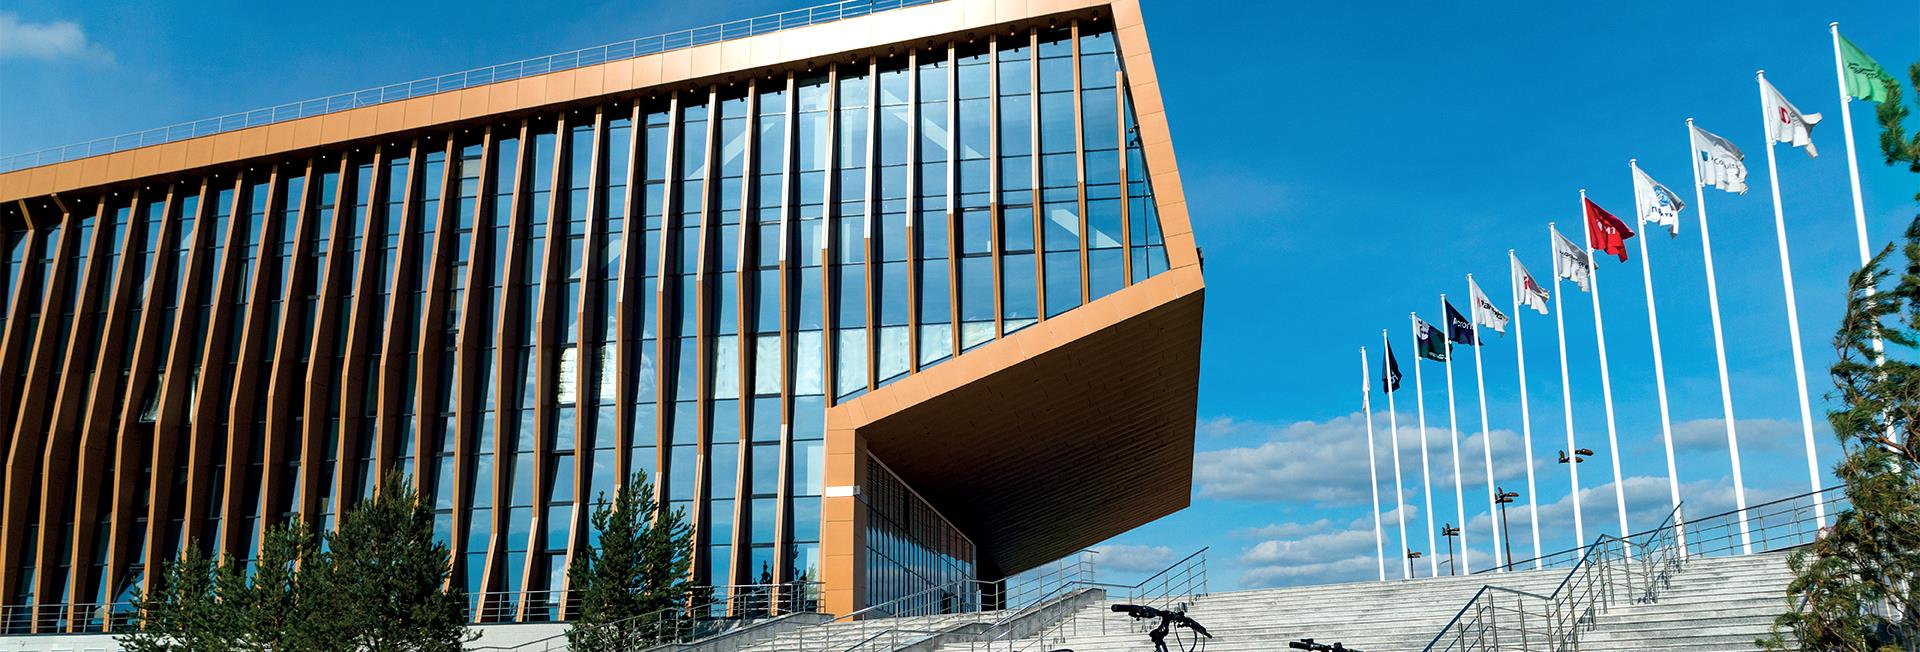
\includegraphics[width=\paperwidth,height=0.58\paperheight]{assets/innopolis-campus.jpg}};
    \fill[white] (current page.south west) rectangle
      ([yshift=-0.58\paperheight]current page.north east);
    \fill[PhysicsBlue] (current page.south west) rectangle
      ([xshift=0.012\paperwidth,yshift=-0.58\paperheight]current page.north west);
    \node[anchor=north west,text width=0.86\paperwidth,align=left]
      at ([xshift=0.055\paperwidth,yshift=-0.64\paperheight]current page.north west) {
      {\color{PhysicsBlue}\small\bfseries MECHANICS PRACTICE SESSION\par}
      \vspace{0.45em}
      {\color{PhysicsInk}\fontsize{17}{20}\selectfont\bfseries Motions in 2 and 3 Dimensions\par}
      \vspace{0.55em}
      {\color{PhysicsMuted}\small Lab 2 · \labversionlabel\par}};
    \node[anchor=east,inner sep=0pt]
      at ([xshift=-0.055\paperwidth,yshift=0.16\paperheight]current page.south east) {
      
\includegraphics[width=0.20\paperwidth]{assets/innopolis-university-logo.png}};
  \end{tikzpicture}
\end{frame}

% C02 — F1, with a quadrant-aware inverse and explicit angle convention.
\begin{frame}{Cartesian and Spherical Coordinates}
  \slidetag{COORDINATE REFERENCE}
  \small
  $\theta$ is measured from $+z$; $\phi$ is measured from $+x$ in the $xy$ plane.
  \begin{columns}[T,onlytextwidth]
    \begin{column}{0.34\textwidth}
      \begin{block}{Spherical to Cartesian}
        \[
          \begin{aligned}
            x&=r\sin\theta\cos\phi,\\
            y&=r\sin\theta\sin\phi,\\
            z&=r\cos\theta.
          \end{aligned}
        \]
      \end{block}
    \end{column}
    \begin{column}{0.27\textwidth}
      \centering
      \resizebox{\linewidth}{!}{\begin{tikzpicture}[
  x={(-0.85cm,-0.45cm)},y={(1cm,0cm)},z={(0cm,1cm)},
  every node/.style={font=\small\sffamily},
  axis/.style={physics line,-{Latex[length=2mm]}},
  guide/.style={PhysicsMuted,densely dashed,line width=0.8pt}
]
  % A right-handed Cartesian frame viewed from the positive octant.
  % The point is generic: r=2.6, theta=48 deg, phi=60 deg for drawing only.
  \coordinate (O) at (0,0,0);
  \coordinate (P) at ({2.6*sin(48)*cos(60)},
    {2.6*sin(48)*sin(60)},{2.6*cos(48)});
  \coordinate (Q) at ({2.6*sin(48)*cos(60)},
    {2.6*sin(48)*sin(60)},0);
  \draw[axis] (O) -- (1.9,0,0) node[below left] {$x$};
  \draw[axis] (O) -- (0,2.0,0) node[right] {$y$};
  \draw[axis] (O) -- (0,0,2.5) node[above] {$z$};
  \draw[guide] (O) -- (Q) -- (P);
  \draw[physics force,PhysicsBlue] (O) -- (P)
    node[pos=0.72,above left,physics label] {$r$};
  \draw[physics accent] plot[variable=\a,domain=0:48,samples=25]
    ({0.88*sin(\a)*cos(60)},{0.88*sin(\a)*sin(60)},
      {0.88*cos(\a)});
  \node[physics label] at (0.08,0.22,0.91) {$\theta$};
  \draw[physics accent] plot[variable=\a,domain=0:60,samples=25]
    ({0.73*cos(\a)},{0.73*sin(\a)},0);
  \node[physics label] at (0.93,0.70,-0.23) {$\phi$};
  \fill[PhysicsInk] (P) circle[radius=1.7pt];
  \node[above right] at (P) {$P$};
  \node[above left,xshift=-3pt,yshift=1pt] at (O) {$O$};
  \node[below right,physics label] at (Q) {$P_{xy}$};
\end{tikzpicture}
}
    \end{column}
    \begin{column}{0.35\textwidth}
      \begin{block}{Cartesian to Spherical}
        \[
          \begin{aligned}
            r&=\sqrt{x^2+y^2+z^2},\\
            \theta&=\arccos(z/r),\\
            \phi&=\operatorname{atan2}(y,x).
          \end{aligned}
        \]
      \end{block}
    \end{column}
  \end{columns}
  \footnotesize
  \textbf{What is $\operatorname{atan2}(y,x)$?}
  It is the two-argument arctangent: it uses the signs of both $x$ and $y$
  to choose the correct quadrant, including when $x=0$ and $y\ne0$.
  For example, $\operatorname{atan2}(1,-1)=135^\circ$.

  Choose $0\le\theta\le\pi$ and wrap $\phi$ into $[0,2\pi)$.
  The azimuth is undefined on the $z$ axis; both angles are undefined at $r=0$.
\end{frame}

% C03 — explicit quadrant-aware calculation requested in the draft revision.
\begin{frame}{Calculating the Two-Argument Arctangent}
  \slidetag{COORDINATE REFERENCE}
  \small
  The signs of $x$ and $y$ determine the quadrant. For $-\pi<\alpha\le\pi$,
  \[
    \alpha=\operatorname{atan2}(y,x)=
    \begin{cases}
      \arctan(y/x),      & x>0,\\
      \arctan(y/x)+\pi,  & x<0,\ y\ge0,\\
      \arctan(y/x)-\pi,  & x<0,\ y<0,\\
      \pi/2,            & x=0,\ y>0,\\
      -\pi/2,           & x=0,\ y<0.
    \end{cases}
  \]
  Here $\arctan$ returns angles in $(-\pi/2,\pi/2)$;
  $\operatorname{atan2}(0,0)$ is undefined.
  \begin{block}{Use the spherical-coordinate range $0\le\phi<2\pi$}
    Set $\phi=\alpha$ if $\alpha\ge0$; otherwise set $\phi=\alpha+2\pi$.
  \end{block}
\end{frame}

% P01 — F2--F4 / S1. No length unit was specified in the source.
\begin{frame}{Problem 1 — Distance Between Two Points}
  \slidetag{PROBLEM 1}
  Two points are described using different coordinate systems:
  \begin{columns}[T,onlytextwidth]
    \begin{column}{0.48\textwidth}
      \begin{block}{Point A: spherical coordinates}
        \[
          \theta=\frac{\pi}{2},\qquad \phi=\frac{\pi}{3},\qquad r=6.
        \]
      \end{block}
    \end{column}
    \begin{column}{0.48\textwidth}
      \begin{block}{Point B: Cartesian coordinates}
        \[
          x=5,\qquad y=5\sqrt{3},\qquad z=0.
        \]
      \end{block}
    \end{column}
  \end{columns}
  \begin{block}{Find}
    Determine the distance $AB$ between the two points.
  \end{block}
  \small
  Use the angle convention from the coordinate reference slide.
  All lengths use the same unspecified length unit.
\end{frame}

\begin{solutionframe}[Solution 1 — Convert the Coordinates]
  \begin{columns}[T,onlytextwidth]
    \begin{column}{0.55\textwidth}
      \textbf{Cartesian components.}
      Convert $A$ before subtracting the coordinates:
      \[
        \begin{aligned}
          x_A&=r\sin\theta\cos\phi\\
             &=6\sin\frac{\pi}{2}\cos\frac{\pi}{3}=3,\\[0.3em]
          y_A&=r\sin\theta\sin\phi\\
             &=6\sin\frac{\pi}{2}\sin\frac{\pi}{3}=3\sqrt3,\\[0.3em]
          z_A&=r\cos\theta=6\cos\frac{\pi}{2}=0.
        \end{aligned}
      \]
    \end{column}
    \begin{column}{0.41\textwidth}
      \centering
      \resizebox{!}{0.44\paperheight}{\begin{tikzpicture}[x=0.40cm,y=0.40cm,
  every node/.style={font=\small\sffamily}]
  \coordinate (O) at (0,0);
  \coordinate (A) at (3,{3*sqrt(3)});
  \coordinate (B) at (5,{5*sqrt(3)});
  \draw[physics line,-{Latex[length=2mm]}] (-0.5,0) -- (7.3,0)
    node[right] {$x$};
  \draw[physics line,-{Latex[length=2mm]}] (0,-0.5) -- (0,9.8)
    node[above] {$y$};
  \draw[physics force,PhysicsBlue] (O) -- (B);
  \draw[PhysicsMuted,densely dashed,line width=0.8pt]
    (3,0) -- (A) (5,0) -- (B);
  \foreach \p in {O,A,B}{\fill[PhysicsInk] (\p) circle[radius=2pt];}
  \node[below left] at (O) {$O$};
  \node[above left,physics label] at (A) {$A$};
  \node[above right,physics label] at (B) {$B$};
  \draw[physics dimension] (1.1,-0.6) -- (4.1,{3*sqrt(3)-0.6})
    node[midway,right=2pt,physics label] {$OA=6$};
  \draw[physics dimension] (-1.0,0.6) -- (4.0,{5*sqrt(3)+0.6})
    node[pos=0.78,above left,physics label] {$OB=10$};
  \node[physics label] at (4.7,1.0) {$z=0$};
\end{tikzpicture}
}
      \answer{\(A=(3,3\sqrt3,0).\)}
    \end{column}
  \end{columns}
\end{solutionframe}

\begin{solutionframe}[Solution 1 — Use the Displacement Vector]
  \begin{columns}[T,onlytextwidth]
    \begin{column}{0.55\textwidth}
      Subtract the position of $A$ from the position of $B$:
      \[
        \begin{aligned}
          \overrightarrow{AB}&=\mathbf r_B-\mathbf r_A\\
            &=(5-3,\,5\sqrt3-3\sqrt3,\,0)\\
            &=(2,2\sqrt3,0).
        \end{aligned}
      \]
      The distance is the magnitude of the displacement:
      \[
        AB=\sqrt{(\Delta x)^2+(\Delta y)^2+(\Delta z)^2}.
      \]
    \end{column}
    \begin{column}{0.41\textwidth}
      \centering
      \resizebox{!}{0.44\paperheight}{\begin{tikzpicture}[x=0.40cm,y=0.40cm,
  every node/.style={font=\small\sffamily}]
  \coordinate (O) at (0,0);
  \coordinate (A) at (3,{3*sqrt(3)});
  \coordinate (B) at (5,{5*sqrt(3)});
  \draw[physics line,-{Latex[length=2mm]}] (-0.5,0) -- (7.3,0)
    node[right] {$x$};
  \draw[physics line,-{Latex[length=2mm]}] (0,-0.5) -- (0,9.8)
    node[above] {$y$};
  \draw[physics force,PhysicsBlue] (O) -- (B);
  \draw[PhysicsMuted,densely dashed,line width=0.8pt]
    (3,0) -- (A) (5,0) -- (B);
  \foreach \p in {O,A,B}{\fill[PhysicsInk] (\p) circle[radius=2pt];}
  \node[below left] at (O) {$O$};
  \node[above left,physics label] at (A) {$A$};
  \node[above right,physics label] at (B) {$B$};
  \draw[physics dimension] (1.1,-0.6) -- (4.1,{3*sqrt(3)-0.6})
    node[midway,right=2pt,physics label] {$OA=6$};
  \draw[physics dimension] (-1.0,0.6) -- (4.0,{5*sqrt(3)+0.6})
    node[pos=0.78,above left,physics label] {$OB=10$};
  \node[physics label] at (4.7,1.0) {$z=0$};
\end{tikzpicture}
}
    \end{column}
  \end{columns}
  \answer{\(AB=\sqrt{2^2+(2\sqrt3)^2}=\sqrt{16}=4\) length units.}
\end{solutionframe}

% P02 — F5--F6 / S2. Ideal vertical, spatially uniform rain.
\begin{frame}{Problem 2 — Rain and Moving Trucks}
  \slidetag{PROBLEM 2}
  \small
  Two identical open dump trucks are in the rain. One is at rest; the other
  moves horizontally at constant speed $V$.
  \begin{center}
    \resizebox{0.58\textwidth}{!}{\begin{tikzpicture}[x=1cm,y=1cm,
  every node/.style={font=\small\sffamily}]
  % Identical open bodies; the dotted segment marks each horizontal aperture.
  \foreach \shift/\title in {0/At rest,5.5/Moving}{
    \begin{scope}[xshift=\shift cm]
      \node[font=\small\sffamily\bfseries] at (1.7,3.2) {\title};
      \foreach \x in {0.3,0.75,...,3.5}{
        \draw[PhysicsBlue,-{Latex[length=1.6mm]},line width=0.85pt]
          (\x,2.75) -- (\x,2.23);
      }
      \draw[physics line,fill=PhysicsPaper]
        (0.15,1.8) -- (0.3,0.95) -- (2.2,0.95) -- (2.3,1.8);
      \draw[PhysicsMuted,densely dotted,line width=0.9pt]
        (0.15,1.8) -- (2.3,1.8);
      \draw[physics line,fill=PhysicsPaper]
        (2.5,0.7) -- (2.5,1.62) -- (3.1,1.62) -- (3.58,1.1)
        -- (3.68,0.7) -- cycle;
      \draw[physics line] (2.63,1.5) -- (3.02,1.5) -- (3.33,1.14)
        -- (2.63,1.14) -- cycle;
      \draw[physics line] (0.2,0.7) -- (3.7,0.7);
      \foreach \x in {0.75,1.85,3.14}{
        \draw[physics line,fill=white] (\x,0.55) circle[radius=0.24];
      }
      \draw[PhysicsLine,line width=1.0pt] (-0.1,0.29) -- (4.2,0.29);
    \end{scope}
  }
  \node at (1.8,-0.12) {$V=0$};
  \draw[physics force,PhysicsBlue] (6.2,-0.1) -- (8.3,-0.1)
    node[midway,below=2pt] {$V=\mathrm{const}$};
\end{tikzpicture}
}
  \end{center}
  \begin{block}{Find}
    Which truck collects more rainwater through its open top per minute?
  \end{block}
  \footnotesize
  Model: uniform vertical rain and equal horizontal openings.
  Neglect airflow disturbances, splashing, and water entering through the sides.
\end{frame}

\begin{solutionframe}[Solution 2 — Compare Collected Volumes]
  \begin{columns}[T,onlytextwidth]
    \begin{column}{0.46\textwidth}
      \textbf{Equal collection volumes.}
      Let $S$ be the opening area and $v_r$ the downward rain speed.

      Over a time $T$, the collected drops initially occupy a prism
      of vertical height $v_rT$.

      Motion shears this prism horizontally by $VT$; its base area
      and vertical height stay the same. Therefore,
      \[
        \mathcal V_{\rm rest}=\mathcal V_{\rm moving}=S v_rT.
      \]
    \end{column}
    \begin{column}{0.50\textwidth}
      \centering
      \resizebox{\linewidth}{!}{\begin{tikzpicture}[x=1cm,y=1cm,
  every node/.style={font=\small\sffamily}]
  % Ground-frame collection volumes at the start of the interval T.
  % A drop at height v_r*t enters the aperture displaced by V*t.
  % Both prisms have an identical base area S and transverse depth.
  \foreach \shift/\shear/\title in {0/0/At rest,3.3/0.8/Moving}{
    \begin{scope}[xshift=\shift cm]
      \coordinate (a) at (0,0);
      \coordinate (b) at (1.3,0);
      \coordinate (c) at (1.65,0.28);
      \coordinate (d) at (0.35,0.28);
      \coordinate (aa) at (\shear,2.05);
      \coordinate (bb) at ({1.3+\shear},2.05);
      \coordinate (cc) at ({1.65+\shear},2.33);
      \coordinate (dd) at ({0.35+\shear},2.33);
      \fill[PhysicsCyan!24] (a) -- (b) -- (bb) -- (aa) -- cycle;
      \fill[PhysicsCyan!40] (b) -- (c) -- (cc) -- (bb) -- cycle;
      \fill[PhysicsCyan!20] (aa) -- (bb) -- (cc) -- (dd) -- cycle;
      \draw[physics accent] (a) -- (b) -- (c) -- (cc) -- (dd)
        -- (aa) -- (a) (aa) -- (bb) -- (cc) (b) -- (bb);
      \draw[PhysicsMuted,densely dashed,line width=0.8pt]
        (a) -- (d) -- (c) (d) -- (dd);
      \node[physics label] at (0.8,-0.25) {$S$};
      \node[font=\small\sffamily\bfseries] at (0.9,-0.72) {\title};
    \end{scope}
  }
  \draw[physics dimension] (-0.45,0) -- (-0.45,2.05)
    node[midway,left,physics label] {$v_rT$};
  \draw[physics dimension] (6.05,0) -- (6.05,2.05)
    node[midway,right,physics label] {$v_rT$};
  \draw[PhysicsMuted,densely dashed,line width=0.7pt]
    (3.3,0) -- (3.3,2.76) (4.1,2.05) -- (4.1,2.76);
  \draw[physics dimension] (3.3,2.65) -- (4.1,2.65)
    node[midway,above,physics label] {$VT$};
  \node[text=PhysicsMuted] at (2.9,-1.2) {Same transverse width; schematic};
\end{tikzpicture}
}
    \end{column}
  \end{columns}
  \answer{Equal collection volumes contain equal water amounts:
    both trucks collect the same amount per minute.}
\end{solutionframe}

% P03 — F7--F8 / S3. Source vector arrangement and Pythagorean solution.
\begin{frame}{Problem 3 — Flying North in a Wind}
  \slidetag{PROBLEM 3}
  \begin{columns}[T,onlytextwidth]
    \begin{column}{0.55\textwidth}
      \small
      A plane has an airspeed of $v_{PA}=\SI{120}{\kilo\metre\per\hour}$.
      The wind blows from the northeast at
      $v_{AE}=\SI{40}{\kilo\metre\per\hour}$, toward the southwest
      at $\ang{45}$ to the east--west line.
      The pilot wants to travel due north relative to the ground.
      \begin{block}{Find}
        \begin{enumerate}
          \item The heading angle $\theta$, measured east of north.
          \item The ground speed $v_{PE}$.
        \end{enumerate}
      \end{block}
      \footnotesize
      $P$: plane, $A$: air, $E$: Earth.
    \end{column}
    \begin{column}{0.41\textwidth}
      \centering
      \resizebox{!}{0.48\paperheight}{\begin{tikzpicture}[x=1cm,y=1cm,
  every node/.style={font=\small\sffamily}]
  % F7 arrangement, with equal x/y scaling and the correct wind arrow.
  % Wind W->O, airspeed O->P, ground velocity W->P.
  \coordinate (O) at (0,0);
  \coordinate (W) at (1,1);
  \coordinate (P) at (1,{sqrt(17)});
  \draw[PhysicsMuted,densely dashed,line width=0.8pt,-{Latex[length=2mm]}]
    (0,0) -- (0,4.65) node[above] {North};
  \draw[PhysicsMuted,densely dashed,line width=0.8pt,-{Latex[length=2mm]}]
    (0,0) -- (2.3,0) node[right] {East};
  \draw[physics force,PhysicsBlue,line width=1.6pt] (O) -- (P)
    node[pos=0.74,left=5pt,physics label] {$\vec v_{PA}$};
  \draw[physics force,PhysicsNavy] (W) -- (O)
    node[pos=0.35,above left=1pt,physics label] {$\vec v_{AE}$};
  \draw[physics force,dashed,line width=1.4pt] (W) -- (P)
    node[pos=0.47,right=5pt,physics label] {$\vec v_{PE}$};
  \draw[physics accent] (0,1.9)
    arc[start angle=90,end angle={atan(sqrt(17))},radius=1.9];
  \node[physics label] at (0.23,2.2) {$\theta$};
  \draw[physics accent] (0.62,0) arc[start angle=0,end angle=45,radius=0.62];
  \node[physics label] at (0.88,0.25) {$45^\circ$};
  \fill[PhysicsInk] (O) circle[radius=1.7pt];
\end{tikzpicture}
}
    \end{column}
  \end{columns}
\end{frame}

\begin{solutionframe}[Solution 3 — Use the Velocity Triangle]
  \begin{columns}[T,onlytextwidth]
    \begin{column}{0.58\textwidth}
      The velocities satisfy
      \[
        \vec v_{PE}=\vec v_{PA}+\vec v_{AE}.
      \]
      The right triangle has hypotenuse $v_{PA}$ and legs
      $v_{AE}\sin\ang{45}$ and $v_{PE}+v_{AE}\cos\ang{45}$.
      By Pythagoras,
      \[
        \begin{aligned}
          &(v_{PE}+v_{AE}\cos\ang{45})^2\\
          &\qquad +(v_{AE}\sin\ang{45})^2=v_{PA}^2.
        \end{aligned}
      \]
      Hence, with speeds in \si{\kilo\metre\per\hour},
      \[
        v_{PE}=\sqrt{120^2-(40\sin\ang{45})^2}-40\cos\ang{45}.
      \]
    \end{column}
    \begin{column}{0.38\textwidth}
      \centering
      \resizebox{!}{0.46\paperheight}{\begin{tikzpicture}[x=1cm,y=1cm,
  every node/.style={font=\small\sffamily}]
  % F7 arrangement, with equal x/y scaling and the correct wind arrow.
  % Wind W->O, airspeed O->P, ground velocity W->P.
  \coordinate (O) at (0,0);
  \coordinate (W) at (1,1);
  \coordinate (P) at (1,{sqrt(17)});
  \draw[PhysicsMuted,densely dashed,line width=0.8pt,-{Latex[length=2mm]}]
    (0,0) -- (0,4.65) node[above] {North};
  \draw[PhysicsMuted,densely dashed,line width=0.8pt,-{Latex[length=2mm]}]
    (0,0) -- (2.3,0) node[right] {East};
  \draw[physics force,PhysicsBlue,line width=1.6pt] (O) -- (P)
    node[pos=0.74,left=5pt,physics label] {$\vec v_{PA}$};
  \draw[physics force,PhysicsNavy] (W) -- (O)
    node[pos=0.35,above left=1pt,physics label] {$\vec v_{AE}$};
  \draw[physics force,dashed,line width=1.4pt] (W) -- (P)
    node[pos=0.47,right=5pt,physics label] {$\vec v_{PE}$};
  \draw[physics accent] (0,1.9)
    arc[start angle=90,end angle={atan(sqrt(17))},radius=1.9];
  \node[physics label] at (0.23,2.2) {$\theta$};
  \draw[physics accent] (0.62,0) arc[start angle=0,end angle=45,radius=0.62];
  \node[physics label] at (0.88,0.25) {$45^\circ$};
  \fill[PhysicsInk] (O) circle[radius=1.7pt];
\end{tikzpicture}
}
    \end{column}
  \end{columns}
  \answer{The ground speed is $v_{PE}\approx\SI{88.3}{\kilo\metre\per\hour}$.}
\end{solutionframe}

\begin{solutionframe}[Solution 3 — Find the Heading Angle]
  \begin{columns}[T,onlytextwidth]
    \begin{column}{0.55\textwidth}
      From the same right triangle,
      \[
        \sin\theta=\frac{v_{AE}\sin\ang{45}}{v_{PA}}.
      \]
      Substitute the two given speeds:
      \[
        \theta=\arcsin\!\left(\frac{40\sin\ang{45}}{120}\right)
          \approx\ang{13.6}.
      \]
      The pilot must head east of north to compensate for the westward wind.
    \end{column}
    \begin{column}{0.41\textwidth}
      \centering
      \resizebox{!}{0.44\paperheight}{\begin{tikzpicture}[x=1cm,y=1cm,
  every node/.style={font=\small\sffamily}]
  % F7 arrangement, with equal x/y scaling and the correct wind arrow.
  % Wind W->O, airspeed O->P, ground velocity W->P.
  \coordinate (O) at (0,0);
  \coordinate (W) at (1,1);
  \coordinate (P) at (1,{sqrt(17)});
  \draw[PhysicsMuted,densely dashed,line width=0.8pt,-{Latex[length=2mm]}]
    (0,0) -- (0,4.65) node[above] {North};
  \draw[PhysicsMuted,densely dashed,line width=0.8pt,-{Latex[length=2mm]}]
    (0,0) -- (2.3,0) node[right] {East};
  \draw[physics force,PhysicsBlue,line width=1.6pt] (O) -- (P)
    node[pos=0.74,left=5pt,physics label] {$\vec v_{PA}$};
  \draw[physics force,PhysicsNavy] (W) -- (O)
    node[pos=0.35,above left=1pt,physics label] {$\vec v_{AE}$};
  \draw[physics force,dashed,line width=1.4pt] (W) -- (P)
    node[pos=0.47,right=5pt,physics label] {$\vec v_{PE}$};
  \draw[physics accent] (0,1.9)
    arc[start angle=90,end angle={atan(sqrt(17))},radius=1.9];
  \node[physics label] at (0.23,2.2) {$\theta$};
  \draw[physics accent] (0.62,0) arc[start angle=0,end angle=45,radius=0.62];
  \node[physics label] at (0.88,0.25) {$45^\circ$};
  \fill[PhysicsInk] (O) circle[radius=1.7pt];
\end{tikzpicture}
}
    \end{column}
  \end{columns}
  \answer{Heading: $\theta\approx\ang{13.6}$ east of north.\\
    Ground speed: $v_{PE}\approx\SI{88.3}{\kilo\metre\per\hour}$.}
\end{solutionframe}

% P04 — F9--F11 / S4. Both graphs belong to the shared problem statement.
\begin{frame}{Problem 4 — Read the Direction Graph}
  \slidetag{PROBLEM 4}
  \small
  A particle's position is
  \[
    \vec r(t)=5t\,\hat{\imath}+(c_1t+c_2t^2)\,\hat{\jmath},
    \qquad \vec r\text{ in metres},\quad t\text{ in seconds}.
  \]
  The unit vectors $\hat{\imath}$ and $\hat{\jmath}$ point along $+x$ and $+y$.
  The angle $\theta$ is measured from $+x$ to $\vec r$.
  \begin{columns}[T,onlytextwidth]
    \begin{column}{0.45\textwidth}
      \centering
      \resizebox{!}{0.36\paperheight}{\begin{tikzpicture}[x=1cm,y=1cm,
  every node/.style={font=\small\sffamily}]
  % Generic vector; theta is measured from +x, not from +y.
  \coordinate (O) at (0,0);
  \coordinate (P) at (3.5,2.45);
  \draw[physics line,-{Latex[length=2mm]}] (-0.2,0) -- (4.2,0)
    node[right] {$x$};
  \draw[physics line,-{Latex[length=2mm]}] (0,-0.2) -- (0,3.15)
    node[above] {$y$};
  \draw[PhysicsMuted,densely dashed,line width=0.8pt]
    (0,2.45) -- (P) -- (3.5,0);
  \draw[physics force,PhysicsBlue] (O) -- (P)
    node[pos=0.68,above left,physics label] {$\vec r(t)$};
  \draw[physics accent] (0.9,0)
    arc[start angle=0,end angle={atan(2.45/3.5)},radius=0.9];
  \node[physics label] at (1.28,0.38) {$\theta$};
  \draw[physics force,PhysicsNavy] (O) -- (0.75,0)
    node[midway,below=3pt] {$\hat{\imath}$};
  \draw[physics force,PhysicsNavy] (O) -- (0,0.75)
    node[midway,left=3pt] {$\hat{\jmath}$};
  \node[below=3pt] at (3.5,0) {$x(t)$};
  \node[left=3pt] at (0,2.45) {$y(t)$};
  \node[below left=3pt] at (O) {$O$};
  \fill[PhysicsInk] (P) circle[radius=1.7pt];
\end{tikzpicture}
}
      \begin{block}{Find}
        Determine the constants $c_1$ and $c_2$.
      \end{block}
    \end{column}
    \begin{column}{0.51\textwidth}
      \centering
      \resizebox{!}{0.46\paperheight}{\begin{tikzpicture}
  \begin{axis}[
    width=6.7cm,height=5.2cm,
    xmin=0,xmax=20,ymin=-25,ymax=40,
    axis lines=left,
    axis line style={PhysicsNavy,-{Latex[length=2mm]}},
    xtick={0,5,10,15,20},ytick={-20,0,20,40},
    minor x tick num=4,minor y tick num=3,
    xlabel={$t$ (\si{\second})},ylabel={$\theta$ (deg)},
    tick label style={font=\small\sffamily},
    label style={font=\small\sffamily},
    grid=both,
    major grid style={PhysicsMuted!50,line width=0.5pt},
    minor grid style={PhysicsLine,line width=0.4pt},
    clip=false
  ]
    % Visual reconstruction of F9: the drawn shape is not new exact data.
    \draw[physics line,line width=1.5pt]
      (axis cs:0,35)
      .. controls (axis cs:4,27.5) and (axis cs:8,17.2) .. (axis cs:10,11.4)
      .. controls (axis cs:12,5.8) and (axis cs:13,2.9) .. (axis cs:14,0)
      .. controls (axis cs:16,-5.7) and (axis cs:18,-11.6) .. (axis cs:20,-17.3);
    \draw[PhysicsMuted,line width=0.7pt] (axis cs:0,0) -- (axis cs:20,0);
    \draw[PhysicsNavy,fill=white,line width=1.0pt]
      (axis cs:0,35) circle[radius=2.6pt];
    \node[anchor=south east,font=\small\sffamily,text=PhysicsMuted]
      at (axis description cs:1,1.025) {Source graph (redrawn)};
  \end{axis}
\end{tikzpicture}
}
      \par\footnotesize
      Open endpoint: initial direction just after motion begins.
    \end{column}
  \end{columns}
\end{frame}

\begin{solutionframe}[Solution 4 — From the Vector to Coordinates]
  Compare the position vector with its Cartesian form:
  \[
    \begin{aligned}
      \vec r(t)&=x(t)\,\hat{\imath}+y(t)\,\hat{\jmath}\\
         &=5t\,\hat{\imath}+(c_1t+c_2t^2)\,\hat{\jmath}.
    \end{aligned}
  \]
  The coefficients of the unit vectors give
  \[
    x(t)=5t,\qquad y(t)=c_1t+c_2t^2.
  \]
  From the right triangle in the problem statement, for $t>0$,
  \[
    \tan\theta=\frac{y(t)}{x(t)}
      =\frac{c_1t+c_2t^2}{5t}=\frac{c_1+c_2t}{5}.
  \]
  \footnotesize
  Use metres and seconds throughout, as in the given position formula.
\end{solutionframe}

\begin{solutionframe}[Solution 4 — Read Two Points from the Graph]
  \begin{columns}[T,onlytextwidth]
    \begin{column}{0.55\textwidth}
      Extrapolate the initial angle from the graph:
      \[
        \tan\ang{35}\approx\frac{c_1}{5}
        \quad\Rightarrow\quad c_1\approx5\tan\ang{35}\approx3.5.
      \]
      At $t=\SI{14}{\second}$, the angle is zero:
      \[
        0=\frac{c_1+14c_2}{5}
        \quad\Rightarrow\quad c_2\approx-\frac{3.5}{14}=-0.25.
      \]
      \footnotesize
      The initial angle describes the start of the curve; at exactly $t=0$
      the position vector is zero and has no direction.
    \end{column}
    \begin{column}{0.41\textwidth}
      \centering
      \resizebox{\linewidth}{!}{\begin{tikzpicture}
  \begin{axis}[
    width=6.7cm,height=5.2cm,
    xmin=0,xmax=20,ymin=-25,ymax=40,
    axis lines=left,
    axis line style={PhysicsNavy,-{Latex[length=2mm]}},
    xtick={0,5,10,15,20},ytick={-20,0,20,40},
    minor x tick num=4,minor y tick num=3,
    xlabel={$t$ (\si{\second})},ylabel={$\theta$ (deg)},
    tick label style={font=\small\sffamily},
    label style={font=\small\sffamily},
    grid=both,
    major grid style={PhysicsMuted!50,line width=0.5pt},
    minor grid style={PhysicsLine,line width=0.4pt},
    clip=false
  ]
    % PGF trigonometric functions return degrees. Rounded c1 and c2 are used.
    \addplot[PhysicsBlue,line width=1.5pt,domain=0.001:20,samples=100]
      {atan((3.5-0.25*x)/5)};
    \draw[PhysicsMuted,line width=0.7pt] (axis cs:0,0) -- (axis cs:20,0);
    \draw[PhysicsBlue,fill=white,line width=1.0pt]
      (axis cs:0,{atan(0.7)}) circle[radius=2.6pt];
    \fill[PhysicsBlue] (axis cs:14,0) circle[radius=2.3pt];
    \draw[PhysicsBlue,densely dashed,line width=0.8pt]
      (axis cs:14,-25) -- (axis cs:14,0);
    \node[anchor=south west,physics label,text=PhysicsBlue]
      at (axis cs:0.8,34) {$\theta\approx35^\circ$ initially};
    \node[anchor=north east,physics label,text=PhysicsBlue]
      at (axis cs:13.6,-2) {$\approx\SI{14}{\second}$};
    \node[anchor=south east,font=\small\sffamily,text=PhysicsMuted]
      at (axis description cs:1,1.025) {Calculated check};
  \end{axis}
\end{tikzpicture}
}
    \end{column}
  \end{columns}
  \answer{$c_1\approx\SI{3.5}{\metre\per\second}$,
    \qquad $c_2\approx-\SI{0.25}{\metre\per\second\squared}$.}
\end{solutionframe}

% P05 — F12--F14 / S5. g=9.8 is the same explicit convention as in Lab 1.
\begin{frame}{Problem 5 — Can the Ball Escape the Pit?}
  \slidetag{PROBLEM 5}
  \begin{columns}[T,onlytextwidth]
    \begin{column}{0.53\textwidth}
      \small
      A ball is thrown from the bottom of a rectangular pit with initial speed
      $v_0=\SI{20}{\metre\per\second}$ at $\alpha=\ang{60}$ above the horizontal.
      The pit is $h=\SI{10}{\metre}$ deep. The wall in the direction of the throw
      is $L=\SI{10}{\metre}$ away.
      \begin{block}{Find}
        Will the ball escape the pit?
      \end{block}
      \footnotesize
      Model the ball as a particle, neglect air resistance, and use
      $g=\SI{9.8}{\metre\per\second\squared}$.
    \end{column}
    \begin{column}{0.43\textwidth}
      \centering
      \resizebox{\linewidth}{!}{\begin{tikzpicture}[
  x=1cm,y=1cm,font=\normalsize\sffamily,
  every node/.style={text=PhysicsInk},
  velocity/.style={-{Latex[length=3mm]},PhysicsBlue,line width=1.5pt}
]
  % G08: equal physical lengths h and L have equal drawing lengths.
  % No trajectory is shown on the problem slide.
  \coordinate (O) at (0,0);
  \coordinate (W) at (3.2,3.2);
  \fill[PhysicsPaper] (-0.14,3.2) -- (-0.14,-0.14) --
    (3.34,-0.14) -- (3.34,3.2) -- (W) -- (3.2,0) --
    (O) -- (0,3.2) -- cycle;
  \draw[physics line,line width=1.5pt] (0,3.2) -- (O) -- (3.2,0) -- (W);
  \fill[PhysicsNavy] (O) circle[radius=2.5pt];
  \draw[velocity] (O) -- (60:2.25) node[above right] {$v_0$};
  \draw[PhysicsMuted,line width=0.8pt] (0.8,0) arc[start angle=0,end angle=60,radius=0.8];
  \node at (1.15,0.38) {$60^\circ$};
  \draw[PhysicsMuted,thin] (0,-0.2) -- (0,-0.68);
  \draw[PhysicsMuted,thin] (3.2,-0.2) -- (3.2,-0.68);
  \draw[physics dimension,line width=0.8pt] (0,-0.51) --
    node[below=4pt] {$L=\SI{10}{\metre}$} (3.2,-0.51);
  \draw[PhysicsMuted,thin] (3.42,0) -- (3.86,0);
  \draw[PhysicsMuted,thin] (3.42,3.2) -- (3.86,3.2);
  \draw[physics dimension,line width=0.8pt] (3.69,0) --
    node[right=4pt] {$h=\SI{10}{\metre}$} (3.69,3.2);
\end{tikzpicture}
}
    \end{column}
  \end{columns}
\end{frame}

\begin{solutionframe}[Solution 5 — Reach the Wall]
  \begin{columns}[T,onlytextwidth]
    \begin{column}{0.55\textwidth}
      Choose the origin at release and $+y$ upward.
      Resolve the initial velocity:
      \[
        v_{0x}=v_0\cos\alpha,\qquad v_{0y}=v_0\sin\alpha.
      \]
      Horizontal motion is uniform. Setting $x=L$ gives the time at the wall:
      \[
        x(t)=v_0\cos\alpha\,t,
        \qquad t_L=\frac{L}{v_0\cos\alpha}.
      \]
    \end{column}
    \begin{column}{0.41\textwidth}
      \centering
      \resizebox{\linewidth}{!}{\begin{tikzpicture}[
  x=1cm,y=1cm,font=\normalsize\sffamily,
  every node/.style={text=PhysicsInk},
  velocity/.style={-{Latex[length=3mm]},PhysicsBlue,line width=1.5pt}
]
  % G08: equal physical lengths h and L have equal drawing lengths.
  % No trajectory is shown on the problem slide.
  \coordinate (O) at (0,0);
  \coordinate (W) at (3.2,3.2);
  \fill[PhysicsPaper] (-0.14,3.2) -- (-0.14,-0.14) --
    (3.34,-0.14) -- (3.34,3.2) -- (W) -- (3.2,0) --
    (O) -- (0,3.2) -- cycle;
  \draw[physics line,line width=1.5pt] (0,3.2) -- (O) -- (3.2,0) -- (W);
  \fill[PhysicsNavy] (O) circle[radius=2.5pt];
  \draw[velocity] (O) -- (60:2.25) node[above right] {$v_0$};
  \draw[PhysicsMuted,line width=0.8pt] (0.8,0) arc[start angle=0,end angle=60,radius=0.8];
  \node at (1.15,0.38) {$60^\circ$};
  \draw[PhysicsMuted,thin] (0,-0.2) -- (0,-0.68);
  \draw[PhysicsMuted,thin] (3.2,-0.2) -- (3.2,-0.68);
  \draw[physics dimension,line width=0.8pt] (0,-0.51) --
    node[below=4pt] {$L=\SI{10}{\metre}$} (3.2,-0.51);
  \draw[PhysicsMuted,thin] (3.42,0) -- (3.86,0);
  \draw[PhysicsMuted,thin] (3.42,3.2) -- (3.86,3.2);
  \draw[physics dimension,line width=0.8pt] (3.69,0) --
    node[right=4pt] {$h=\SI{10}{\metre}$} (3.69,3.2);
\end{tikzpicture}
}
    \end{column}
  \end{columns}
  \answer{\(\displaystyle
    t_L=\frac{\SI{10}{\metre}}
      {(\SI{20}{\metre\per\second})\cos\ang{60}}
      =\SI{1.0}{\second}.\)}
\end{solutionframe}

\begin{solutionframe}[Solution 5 — Check the Clearance]
  \begin{columns}[T,onlytextwidth]
    \begin{column}{0.55\textwidth}
      Evaluate the vertical position when the ball reaches the wall:
      \[
        y(t)=v_0\sin\alpha\,t-\frac12gt^2.
      \]
      Substituting $t_L=L/(v_0\cos\alpha)$ gives
      \[
        y_L=L\tan\alpha-\frac{gL^2}{2v_0^2\cos^2\alpha}.
      \]
      With $t_L=\SI{1.0}{\second}$,
      \[
        y_L=\bigl(20\sin\ang{60}-4.9\bigr)\,\si{\metre}
          \approx\SI{12.4}{\metre}.
      \]
    \end{column}
    \begin{column}{0.41\textwidth}
      \centering
      \resizebox{\linewidth}{!}{\begin{tikzpicture}[
  x=0.29cm,y=0.29cm,font=\normalsize\sffamily,
  every node/.style={text=PhysicsInk},
  axis/.style={-{Latex[length=2.5mm]},PhysicsMuted,line width=0.8pt}
]
  % G09: physical coordinates in metres; v0=20 m/s, alpha=60 deg, g=9.8 m/s^2.
  % y(x)=sqrt(3)*x-0.049*x^2. Uniform x/y scale is deliberate.
  \pgfmathsetmacro{\wallheight}{sqrt(3)*10-0.049*100}
  \coordinate (O) at (0,0);
  \coordinate (P) at (10,\wallheight);
  \fill[PhysicsPaper] (-0.35,10) -- (-0.35,-0.35) --
    (10.35,-0.35) -- (10.35,10) -- (10,10) -- (10,0) --
    (O) -- (0,10) -- cycle;
  \draw[physics line,line width=1.4pt] (0,10) -- (O) -- (10,0) -- (10,10);
  \draw[axis] (O) -- (15.4,0) node[right] {$x$};
  \draw[axis] (O) -- (0,16.1) node[above] {$y$};
  \draw[PhysicsMuted,dashed,line width=0.8pt] (0,10) -- (12.5,10);
  \node[left=3pt] at (0,10) {$h$};
  \draw[PhysicsMuted,dashed,line width=0.8pt] (0,\wallheight) -- (P);
  \node[left=3pt] at (0,\wallheight) {$y(L)$};
  \draw[physics accent,line width=1.6pt,domain=0:14.7,samples=90]
    plot (\x,{sqrt(3)*\x-0.049*\x*\x});
  \fill[PhysicsBlue] (P) circle[radius=3pt];
  \draw[PhysicsBlue,line width=1pt] (10.8,10) -- (11.65,10);
  \draw[PhysicsBlue,line width=1pt] (10.8,\wallheight) -- (11.65,\wallheight);
  \draw[physics dimension,PhysicsBlue,line width=1pt] (11.25,10) -- (11.25,\wallheight);
  \node[right=4pt] at (11.7,11.25) {clearance};
  \draw[-{Latex[length=2.8mm]},PhysicsBlue,line width=1.2pt]
    (O) -- (3.4,{sqrt(3)*3.4}) node[above left] {$v_0$};
  \fill[PhysicsNavy] (O) circle[radius=2.5pt];
  \node[below left=2pt] at (O) {$O$};
  \node[below=4pt] at (10,0) {$L$};
\end{tikzpicture}
}
    \end{column}
  \end{columns}
  \answer{\(y_L\approx\SI{12.4}{\metre}>h=\SI{10}{\metre}.\)
    Yes, the ball clears the edge and escapes the pit.}
\end{solutionframe}

% P06 — shared problem statement; F15–F16 / S6.
\begin{frame}{Problem 6 — Motion Along a Parabola}
  \slidetag{PROBLEM 6}
  \begin{columns}[T,onlytextwidth]
    \begin{column}{0.53\textwidth}
      \small
      A material point moves with constant speed $v_0$ along
      \[
        y(x)=cx^2,\qquad c>0.
      \]
      At the vertex $x=0$, use
      \[
        \begin{aligned}
          \dot x(t)&=v_0, & \ddot x(t)&=0,\\
          \dot y(t)&=0,   & \ddot y(t)&=a.
        \end{aligned}
      \]
      These values apply at the vertex, where the point moves to the right.
      \begin{block}{Find}
        The acceleration $a$ and radius of curvature $R$ at $x=0$.
      \end{block}
    \end{column}
    \begin{column}{0.43\textwidth}
      \centering
      \resizebox{!}{0.46\paperheight}{\begin{tikzpicture}[
  x=1cm,y=1cm,font=\normalsize\sffamily,
  every node/.style={text=PhysicsInk},
  axis/.style={-{Latex[length=2.5mm]},PhysicsMuted,line width=0.8pt}
]
  % G10: cplot=0.7 is a drawing parameter, never a numerical condition.
  % At x=-1.2 the tangent has slope 2*cplot*x=-1.68.
  \draw[axis] (-2.25,0) -- (2.3,0) node[right] {$x$};
  \draw[axis] (0,-0.25) -- (0,2.95) node[above] {$y$};
  \draw[physics accent,line width=1.6pt,domain=-1.95:1.95,samples=80]
    plot (\x,{0.7*\x*\x});
  \node[right=4pt] at (1.18,1.05) {$y=cx^2$};
  \coordinate (P) at (-1.2,1.008);
  \fill[PhysicsNavy] (P) circle[radius=3pt];
  \draw[-{Latex[length=3mm]},PhysicsNavy,line width=1.4pt]
    (P) -- (-0.7,0.168);
  \node[left=4pt] at (-0.92,0.58) {$v_0$};
  \node[below left=2pt] at (0,0) {$O$};
  \node[anchor=north] at (0,-0.6) {Schematic; $c>0$ shown};
\end{tikzpicture}
}
    \end{column}
  \end{columns}
\end{frame}

% S06A — one source-based derivation, evaluated locally at the vertex.
\begin{solutionframe}[Solution 6 — Acceleration and Radius]
  \small
  \begin{columns}[T,onlytextwidth]
    \begin{column}{0.55\textwidth}
      Differentiate $y(t)=c[x(t)]^2$ twice:
      \[
        \begin{aligned}
          \dot y&=2cx\dot x,\\
          \ddot y&=2c\bigl(\dot x^2+x\ddot x\bigr).
        \end{aligned}
      \]
      At $x=0$, substitute $\dot x=v_0$ and $\ddot y=a$ to obtain
      $a=2cv_0^2$.

      Constant speed means normal acceleration:
      \[
        a=\frac{v_0^2}{R}
        \quad\Longrightarrow\quad R=\frac{1}{2c}.
      \]
    \end{column}
    \begin{column}{0.41\textwidth}
      \centering
      \resizebox{!}{0.40\paperheight}{\begin{tikzpicture}[
  x=1cm,y=1cm,font=\normalsize\sffamily,
  every node/.style={text=PhysicsInk},
  axis/.style={-{Latex[length=2.5mm]},PhysicsMuted,line width=0.8pt}
]
  % G11: cplot=0.7, Rplot=1/(2*cplot). Both axes use the same scale.
  \pgfmathsetmacro{\radiusplot}{1/(2*0.7)}
  \coordinate (O) at (0,0);
  \coordinate (K) at (0,\radiusplot);
  \draw[axis] (-2.1,0) -- (2.3,0) node[right] {$x$};
  \draw[axis] (0,-0.2) -- (0,2.85) node[above] {$y$};
  \draw[PhysicsMuted,dashed,line width=1pt] (K) circle[radius=\radiusplot];
  \draw[physics accent,line width=1.6pt,domain=-1.85:1.85,samples=80]
    plot (\x,{0.7*\x*\x});
  \draw[physics force] (O) -- (0,1.85) node[above left=2pt] {$\vec a$};
  \draw[-{Latex[length=3mm]},PhysicsNavy,line width=1.4pt]
    (O) -- (1.45,0) node[below=5pt] {$v_0$};
  \draw[physics dimension,line width=0.9pt] (K) --
    node[above=3pt] {$R$} (\radiusplot,\radiusplot);
  \fill[PhysicsNavy] (K) circle[radius=2.5pt];
  \node[above left=4pt] at (K) {$K$};
  \fill[PhysicsNavy] (O) circle[radius=2.5pt];
  \node[below left=3pt] at (O) {$O$};
  \node[anchor=north,align=center] at (0,-0.57)
    {Schematic; $c>0$ shown\\$K$: center of curvature};
\end{tikzpicture}
}
    \end{column}
  \end{columns}
  \answer{\(\displaystyle a=2cv_0^2\ \text{(upward)},\qquad R=\frac{1}{2c}.\)}
\end{solutionframe}

% P07 — shared problem statement; F18 / S7. The water is still.
\begin{frame}{Problem 7 — Walking and Swimming}
  \slidetag{PROBLEM 7}\par
  \small
  A traveler walks along the bank from $A$ to $B$ at
  $v_g=\SI{7}{\kilo\metre\per\hour}$, then swims directly to $C$
  at $v_w=\SI{2}{\kilo\metre\per\hour}$. The water is still.
  \begin{columns}[T,onlytextwidth]
    \begin{column}{0.46\textwidth}
      The distances shown are
      \[
        H=\SI{200}{\metre},\qquad L=\SI{45}{\metre}.
      \]
      \begin{block}{Find}
        What distance $AB$ gives the shortest travel time from $A$ to $C$?
      \end{block}
      \footnotesize
      $H$ is measured along the bank; $L$ is the perpendicular distance
      from the bank to $C$.
    \end{column}
    \begin{column}{0.50\textwidth}
      \centering
      \resizebox{!}{0.38\paperheight}{\begin{tikzpicture}[
  x=1cm,y=1cm,font=\normalsize\sffamily,
  every node/.style={text=PhysicsInk},
  route/.style={-{Latex[length=3mm]},line width=1.5pt}
]
  % G12: one uniform scale, H=5.2 and L=1.17 represent 200 m and 45 m.
  % B=3.4 is an illustrative unknown location, not the optimal s.
  \coordinate (A) at (0,0);
  \coordinate (B) at (3.4,0);
  \coordinate (C) at (5.2,1.17);
  \fill[PhysicsBlue!9] (-0.25,0) rectangle (5.55,1.17);
  \fill[PhysicsPaper] (-0.25,-0.24) rectangle (5.55,0);
  \fill[PhysicsPaper] (-0.25,1.17) rectangle (5.55,1.41);
  \draw[physics line] (-0.25,0) -- (5.55,0);
  \draw[physics line] (-0.25,1.17) -- (5.55,1.17);
  \node[text=PhysicsMuted] at (0.9,0.84) {water};
  \draw[route,PhysicsNavy] (A) -- (B) node[midway,above=4pt] {$v_g$};
  \draw[route,PhysicsBlue] (B) -- (C) node[midway,above left=2pt] {$v_w$};
  \draw[PhysicsMuted,dashed,line width=0.8pt] (5.2,0) -- (C);
  \foreach \p in {A,B,C} {\fill[PhysicsNavy] (\p) circle[radius=2.6pt];}
  \node[below left=3pt] at (A) {$A$};
  \node[below=3pt] at (B) {$B$};
  \node[above left=3pt] at (C) {$C$};
  \draw[PhysicsMuted,thin] (0,1.48) -- (0,1.96);
  \draw[PhysicsMuted,thin] (5.2,1.48) -- (5.2,1.96);
  \draw[physics dimension,line width=0.8pt] (0,1.78) --
    node[above=4pt] {$H=\SI{200}{\metre}$} (5.2,1.78);
  \draw[PhysicsMuted,thin] (5.67,0) -- (6.1,0);
  \draw[PhysicsMuted,thin] (5.67,1.17) -- (6.1,1.17);
  \draw[physics dimension,line width=0.8pt] (5.92,0) --
    node[right=4pt] {$L$} (5.92,1.17);
  \draw[physics dimension,line width=0.8pt] (0,-0.65) --
    node[below=4pt] {$s=AB$} (3.4,-0.65);
  \node[anchor=north,text=PhysicsMuted] at (2.6,-1.11) {$B$ is a variable point};
\end{tikzpicture}
}
    \end{column}
  \end{columns}
\end{frame}

% S07A — first source method: stationary travel time, in consistent units.
\begin{solutionframe}[Solution 7 — Minimize the Travel Time]
  \small
  \begin{columns}[T,onlytextwidth]
    \begin{column}{0.53\textwidth}
      Set $s=AB$, with $0\le s\le H$.
      \[
        \begin{aligned}
          BC&=\sqrt{(H-s)^2+L^2},\\
          T(s)&=\frac{s}{v_g}
            +\frac{\sqrt{(H-s)^2+L^2}}{v_w}.
        \end{aligned}
      \]
      Differentiate with respect to $s$:
      \[
        T'(s)=\frac{1}{v_g}
          -\frac{H-s}{v_w\sqrt{(H-s)^2+L^2}}.
      \]
    \end{column}
    \begin{column}{0.43\textwidth}
      \centering
      \resizebox{!}{0.33\paperheight}{\begin{tikzpicture}[
  x=1cm,y=1cm,font=\normalsize\sffamily,
  every node/.style={text=PhysicsInk},
  route/.style={-{Latex[length=3mm]},line width=1.5pt}
]
  % G12: one uniform scale, H=5.2 and L=1.17 represent 200 m and 45 m.
  % B=3.4 is an illustrative unknown location, not the optimal s.
  \coordinate (A) at (0,0);
  \coordinate (B) at (3.4,0);
  \coordinate (C) at (5.2,1.17);
  \fill[PhysicsBlue!9] (-0.25,0) rectangle (5.55,1.17);
  \fill[PhysicsPaper] (-0.25,-0.24) rectangle (5.55,0);
  \fill[PhysicsPaper] (-0.25,1.17) rectangle (5.55,1.41);
  \draw[physics line] (-0.25,0) -- (5.55,0);
  \draw[physics line] (-0.25,1.17) -- (5.55,1.17);
  \node[text=PhysicsMuted] at (0.9,0.84) {water};
  \draw[route,PhysicsNavy] (A) -- (B) node[midway,above=4pt] {$v_g$};
  \draw[route,PhysicsBlue] (B) -- (C) node[midway,above left=2pt] {$v_w$};
  \draw[PhysicsMuted,dashed,line width=0.8pt] (5.2,0) -- (C);
  \foreach \p in {A,B,C} {\fill[PhysicsNavy] (\p) circle[radius=2.6pt];}
  \node[below left=3pt] at (A) {$A$};
  \node[below=3pt] at (B) {$B$};
  \node[above left=3pt] at (C) {$C$};
  \draw[PhysicsMuted,thin] (0,1.48) -- (0,1.96);
  \draw[PhysicsMuted,thin] (5.2,1.48) -- (5.2,1.96);
  \draw[physics dimension,line width=0.8pt] (0,1.78) --
    node[above=4pt] {$H=\SI{200}{\metre}$} (5.2,1.78);
  \draw[PhysicsMuted,thin] (5.67,0) -- (6.1,0);
  \draw[PhysicsMuted,thin] (5.67,1.17) -- (6.1,1.17);
  \draw[physics dimension,line width=0.8pt] (5.92,0) --
    node[right=4pt] {$L$} (5.92,1.17);
  \draw[physics dimension,line width=0.8pt] (0,-0.65) --
    node[below=4pt] {$s=AB$} (3.4,-0.65);
  \node[anchor=north,text=PhysicsMuted] at (2.6,-1.11) {$B$ is a variable point};
\end{tikzpicture}
}\par Use consistent units.
    \end{column}
  \end{columns}
  \begin{block}{Condition for an interior optimum}
    \centering\(\displaystyle
      T'(s)=0
      \quad\to\quad
      \frac{H-s}{\sqrt{(H-s)^2+L^2}}=\frac{v_w}{v_g}.
    \)
  \end{block}
\end{solutionframe}

% S07B — express AB directly and insert the source numbers.
\begin{solutionframe}[Solution 7 — Find the Distance AB]
  \small
  \begin{columns}[T,onlytextwidth]
    \begin{column}{0.55\textwidth}
      Square the condition from the previous slide:
      \[
        v_g^2(H-s)^2=v_w^2\bigl((H-s)^2+L^2\bigr).
      \]
      Collect the terms containing $H-s$:
      \[
        (v_g^2-v_w^2)(H-s)^2=v_w^2L^2.
      \]
      Take the positive root and use $s=AB$:
      \[
        AB=H-\frac{Lv_w}{\sqrt{v_g^2-v_w^2}}.
      \]
    \end{column}
    \begin{column}{0.41\textwidth}
      \centering
      \resizebox{!}{0.33\paperheight}{\begin{tikzpicture}[
  x=1cm,y=1cm,font=\normalsize\sffamily,
  every node/.style={text=PhysicsInk},
  route/.style={-{Latex[length=3mm]},line width=1.5pt}
]
  % G12: one uniform scale, H=5.2 and L=1.17 represent 200 m and 45 m.
  % B=3.4 is an illustrative unknown location, not the optimal s.
  \coordinate (A) at (0,0);
  \coordinate (B) at (3.4,0);
  \coordinate (C) at (5.2,1.17);
  \fill[PhysicsBlue!9] (-0.25,0) rectangle (5.55,1.17);
  \fill[PhysicsPaper] (-0.25,-0.24) rectangle (5.55,0);
  \fill[PhysicsPaper] (-0.25,1.17) rectangle (5.55,1.41);
  \draw[physics line] (-0.25,0) -- (5.55,0);
  \draw[physics line] (-0.25,1.17) -- (5.55,1.17);
  \node[text=PhysicsMuted] at (0.9,0.84) {water};
  \draw[route,PhysicsNavy] (A) -- (B) node[midway,above=4pt] {$v_g$};
  \draw[route,PhysicsBlue] (B) -- (C) node[midway,above left=2pt] {$v_w$};
  \draw[PhysicsMuted,dashed,line width=0.8pt] (5.2,0) -- (C);
  \foreach \p in {A,B,C} {\fill[PhysicsNavy] (\p) circle[radius=2.6pt];}
  \node[below left=3pt] at (A) {$A$};
  \node[below=3pt] at (B) {$B$};
  \node[above left=3pt] at (C) {$C$};
  \draw[PhysicsMuted,thin] (0,1.48) -- (0,1.96);
  \draw[PhysicsMuted,thin] (5.2,1.48) -- (5.2,1.96);
  \draw[physics dimension,line width=0.8pt] (0,1.78) --
    node[above=4pt] {$H=\SI{200}{\metre}$} (5.2,1.78);
  \draw[PhysicsMuted,thin] (5.67,0) -- (6.1,0);
  \draw[PhysicsMuted,thin] (5.67,1.17) -- (6.1,1.17);
  \draw[physics dimension,line width=0.8pt] (5.92,0) --
    node[right=4pt] {$L$} (5.92,1.17);
  \draw[physics dimension,line width=0.8pt] (0,-0.65) --
    node[below=4pt] {$s=AB$} (3.4,-0.65);
  \node[anchor=north,text=PhysicsMuted] at (2.6,-1.11) {$B$ is a variable point};
\end{tikzpicture}
}
    \end{column}
  \end{columns}
  \answer{\(\displaystyle
    AB=\SI{200}{\metre}
      -(\SI{45}{\metre})\frac{2}{\sqrt{7^2-2^2}}
      \approx\SI{187}{\metre}.
  \)}
\end{solutionframe}

% S07C — second source method: compare the rate of shortening with swim speed.
\begin{solutionframe}[Solution 7 — When to Start Swimming]
  \small
  \begin{columns}[T,onlytextwidth]
    \begin{column}{0.53\textwidth}
      While the traveler walks, the remaining swim distance $BC$
      becomes shorter at the rate
      \[
        v_{BC}=v_g\cos\alpha.
      \]
      The angle $\alpha$ lies between the bank and $BC$.
      Multiplying by $\cos\alpha$ gives the component of the walking
      velocity directed toward $C$.

      Keep walking while $v_{BC}>v_w$; start swimming when
      \[
        v_g\cos\alpha=v_w.
      \]
    \end{column}
    \begin{column}{0.43\textwidth}
      \centering
      \resizebox{!}{0.32\paperheight}{\begin{tikzpicture}[
  x=1.7cm,y=1.7cm,font=\normalsize\sffamily,
  every node/.style={text=PhysicsInk}
]
  % G13: schematic projection of walking velocity onto the line BC.
  % B is on the bank; alpha is between the walking direction and BC.
  \pgfmathsetmacro{\routeangle}{atan(1.17/1.8)}
  \pgfmathsetmacro{\projectionx}{1.5*cos(\routeangle)^2}
  \pgfmathsetmacro{\projectiony}{1.5*cos(\routeangle)*sin(\routeangle)}
  \coordinate (B) at (0,0);
  \coordinate (C) at (1.8,1.17);
  \coordinate (V) at (1.5,0);
  \coordinate (Q) at (\projectionx,\projectiony);
  \fill[PhysicsBlue!9] (-0.25,0) rectangle (2.3,1.17);
  \fill[PhysicsPaper] (-0.25,-0.17) rectangle (2.3,0);
  \draw[physics line] (-0.25,0) -- (2.3,0);
  \draw[physics line] (-0.25,1.17) -- (2.3,1.17);
  \draw[PhysicsMuted,dashed,line width=0.9pt] (B) -- (C);
  \draw[PhysicsMuted,dashed,line width=0.9pt] (V) -- (Q);
  \draw[-{Latex[length=3mm]},PhysicsNavy,line width=1.6pt]
    (B) -- (V) node[below=6pt] {$v_g$};
  \draw[-{Latex[length=3mm]},PhysicsBlue,line width=1.7pt]
    (B) -- (Q) node[above left=3pt] {$v_{BC}$};
  \draw[PhysicsNavy,line width=0.9pt] (0.56,0)
    arc[start angle=0,end angle=\routeangle,radius=0.56];
  \node at ({0.77*cos(\routeangle/2)},{0.77*sin(\routeangle/2)}) {$\alpha$};
  \foreach \p in {B,C} {\fill[PhysicsNavy] (\p) circle[radius=2.5pt];}
  \node[below left=4pt] at (B) {$B$};
  \node[above=4pt] at (C) {$C$};
  \node[anchor=north,text=PhysicsMuted] at (1.03,-0.46) {Schematic};
\end{tikzpicture}
}
      \[
        \cos\alpha=\frac{H-AB}{\sqrt{(H-AB)^2+L^2}}.
      \]
    \end{column}
  \end{columns}
  \answer{\(\displaystyle
    AB=H-\frac{Lv_w}{\sqrt{v_g^2-v_w^2}}
      \approx\SI{187}{\metre}.
  \)}
\end{solutionframe}

\end{document}
